\begin{frame}{Programmatic policies}
    \begin{itemize}
        \item \textbf{Differentiable control policies}
        \begin{itemize}
            \item Mainly used for optimization reasons.
            \item In general lack: explainability, compositionality, generalization, inductive bias.
        \end{itemize}
        \item \textbf{Programmatic policies}
        \begin{itemize}
            \item Compositional and inherently explainable.
            \item Domain specific languages provide inductive bias and generalization.
            \item Optimization is very difficult.
        \end{itemize}
    \end{itemize}
    \mybox{0.7, 0.42}{\fullcite{larsenProgrammaticPolicyExtraction2022}}
\end{frame}

\note[itemize]{
    \item I covered the overall motivation for my work, but here's some specific points relating that to this particular work.  
}

\begin{frame}{Approach: Extracting programs from black-box policies}
\begin{itemize}
    \item How to integrate programmatic policy representations with reinforcement learning?
    \item Bellman equation tells us nothing about how to improve a programmatic policy.
    \bigskip
    \item \textbf{Key idea:} Extracting programs from existing policies.
\end{itemize}
\end{frame}

\note[itemize]{
    \item So what can we do? We don't know how to learn directly in program space.
    \item In principle, each program has to be "experimented with" in the environment.
    \item At least, that's the case unless we have a model of how \emph{syntactic} changes result in changes to the agents state distribution and thus obtained reward.
    \item One approach is to bootstrap on existing RL algorithms
    \item Given a trained policy, we can try to extract a program that imitates it.
    \item This has some advantages, such as being compatible with future improvements to RL algorithms.
}

\begin{frame}{Background: Behavioral cloning}
    \begin{itemize}
        \item The simplest way to learn from action demonstrations.
        \item With access to an \emph{expert} $f(x)$, obtain supervised dataset $\{(x_i, f(x_i))\}$.
        \item In RL setting with expert policy $\pi(s)$: Obtain trajectories $\{(s_i, \pi(s_i)\} \sim p_\pi(s)$.
        \item Key issue: Expert only visits \enquote{good} states.
    \end{itemize}
    
    \mybox{0.7, 0.45}{\fullcite{bainFrameworkBehaviouralCloning1999}}
\end{frame}

\note[itemize]{
    \item I'm going to start with some background on methods, building up to my work.
    \item Okay, so how would we go about integrating RL and programs.
    \item The Bellman equation says nothing about improving programs.
    \item It does tell us how to evaluate a given program, though.
    \item The approach here is going to be one where we *somehow* obtain a black-box policy - for example, these days, by using existing Deep RL methods to learn a NN encoding the policy in its weights.
    \item Then, the goal is to extract information from this policy and into a program. That is, we want to obtain a good clone of the black-box policy as a structured program.
    \item There is a really well-known, important problem with BC.
    \item As in any supervised learning problem, the dataset must be representative of the problem.
    \item If we don't have supervision in some part of the state space, the data tells the student nothing about how to act.
    \item Student performance thus degrades as soon as it veers off the expert path.
}

\begin{frame}{Background: Dataset Aggregation}
    \begin{itemize}
        \item Perhaps the first example of \emph{interactive} imitation.
        \item Conceptually simple: At the first iteration, it uses the expert’s policy to gather a dataset of trajectories $\mathcal{D}$ and train a student $\hat\pi_2$ that best mimics the expert on those trajectories. 
        \item Then at iteration $n$, it uses $\hat\pi_n$ to collect more trajectories and adds those trajectories to the dataset $\mathcal{D}$.
    \end{itemize}
    
    \mybox{0.7, 0.42}{\fullcite{rossReductionImitationLearning2011}}
\end{frame}

\note[itemize]{
    \item As I mentioned, this is a well-known issue.
    \item A solution is to do what I would call interactive imitation. Dataset Aggregation or DAgger is an early example of interactive imitation.
    \item It achieves good performance guarantees under the induced state distribution of the final student policy.
    \item It works as follows: <follow screen>
    \item Of course, states are generated by the student in subsequent iterations, BUT actions are still labelled by the expert for the dataset!
}

\begin{frame}[fragile]{Background: Imitation-Projected RL}
\begin{algorithm}[caption={Imitation-Projected Programmatic Reinforcement Learning}]
 input: initial (neural) policy $\pi_0$
 output: joint policy $h_J$, program $p_J$
 $p_0 \leftarrow \textsc{Project}(\pi_0)$
 for $j = 1, \dots, J$
   $h_j \leftarrow \textsc{Update}(p_{j-1}) \quad$ // standard RL algorithm
   $p_j \leftarrow \textsc{Project}(h_j)$
 end
\end{algorithm}

\begin{itemize}
    \item A generic framework for combining RL and structured policies through imitation learning.
\end{itemize}

\mybox{0.7, 0.45}{\fullcite{vermaProgrammaticallyInterpretableReinforcement2018}}
\end{frame}

\note[itemize]{
    \item With that in mind, let's move on to considering structured policies.
    \item Imitation-Projected RL is the starting point for my work with programmatic policies.
    \item It is indeed a framework for the problem that I started this section discussing: imitating a policy with a structured policy. 
    \item It consists of iterating two steps, which we call update and project.
    \item Update takes the current policy and improves it, that is: its a standard RL algorithm.
    \item Project takes this updated policy and projects it into program space.
    \item As the name of the framework suggests, this projection is performed by imitation.
}

\begin{frame}[fragile]{The imitation projector}
The operator $\textsc{Project}$ is implemented using an interactive imitation learning algorithm, here DAgger.

\begin{algorithm}[caption={$\textsc{Project}$: imitation learning}]
 input: structured policy class $\mathcal{P}$
 input: expert policy $h$
 output: structured imitation policy $p_K$
 $\tau_0 \leftarrow $ $N$ on-policy trajectories using $h$
 create supervised dataset $\Gamma_0 = \left\{\left(s, h(s)\right) |\, s \in \tau_0 \right\}$
 $p_0 \leftarrow \textsc{Derive}(\mathcal{P}, \Gamma_0)$
 for $k = 1, \dots, K$
   $\tau_k \leftarrow $ $M$ on-policy trajectories using $p_{k-1}$
   create supervised dataset $\Gamma' = \left\{\left(s, h(s)\right) |\, s \in \tau_k \right\}$
   aggregate datasets: $\Gamma_k = \Gamma_{k-1} \cup \Gamma' \quad$
   $p_k \leftarrow \textsc{Derive}(\mathcal{P}, \Gamma_k)$
 end
\end{algorithm}

\end{frame}

\note[itemize]{
    \item Just to show how DAgger integrates into the imitation projection, here's some pseudocode for PROJECT.
    \item In the framework, $\textsc{Derive}$ is an unspecified function that performs the learning or search for a policy given a dataset.
}



\begin{frame}[fragile]{Imitation-Projection with program synthesis}
\textsc{Derive} was implemented as a search over parameterized PID controllers or simple decision trees.

\begin{itemize}
    \item These spaces are inflexible and small enough to enumerate.
    \item \textbf{Extension 1:} More general, flexible space of programmatic policies.
    \item \textbf{Extension 2:} $\textsc{Derive}$ should improve on previous solutions.
\end{itemize}

\begin{algorithm}[caption={$\textsc{Project}$: imitation learning by improvement}]
 $\dots$
 for $k = 1, \dots, K$
   $\tau_k \leftarrow $ $M$ on-policy trajectories with $p_{k-1}$
   create supervised dataset $\Gamma' = \left\{\left(s, h(s)\right) |\, s \in \tau_k \right\}$
   aggregate datasets: $\Gamma_k = \Gamma_{k-1} \cup \Gamma' \quad$
   $p_k \leftarrow \textsc{Derive}(\Gamma_k, \highlight{\{p_0,\,\dots,\,p_{k-1}\}})$
 end
\end{algorithm}
\end{frame}

\note[itemize]{
    \item Now here's where my contribution comes into play. 
    \item In the paper by Verma, they implement DERIVE as an exhaustive search over some small structured spaces - a set of PID controllers or some small decision trees.
    \item My contributions to this involve two extensions of their work. 
    \item First, we want to use a more general class of policies - namely actual programs from a DSL in the typed lambda calculus.
    \item The first extension obviously causes the search space to be much larger, and so we cannot do exhaustive search or be too naive about it.
    \item That's why my second extension is towards an iterative imitation, where the previously best program is improved in each iteration.
    \item This extension is illustrated here at a high level, where DERIVE now also takes in previous solutions.
}


\newcommand{\Abs}[2]{\mathbb{\lambda}\mathtt{ #1.\,#2}}
\newcommand{\App}[2]{\mathtt{#1\,#2}}
\newcommand{\Sub}[3]{\mathtt{[#1 \mapsto #2]#3}}
\newcommand{\Fun}[2]{\mathtt{#1 \rightarrow #2}}
\newcommand{\Let}[2]{\mathtt{let\, x=#1\,in\, #2}}

\begin{frame}{The lambda calculus}
    \begin{itemize}
        \item A calculus is some rules for manipulating symbols.
        \item The lambda calculus has terms of the form: 
            \begin{itemize}
                \item $\mathtt{t ::= var\,|\, \App{t}{t} \,|\, \Abs{var}{t}}$
            \end{itemize}
        \item Computation is solely done through rewriting terms.
        \item A term of the form $\App{(\Abs{x}{t_{12}})}{t_2}$ is called a \emph{redex}.
        \item The rule $\App{(\Abs{x}{t_{12}})}{t_2} \longrightarrow \Sub{x}{t_2}{t_{12}}$ is called \emph{beta-reduction} and is how function application is defined.
        \item The right hand side reads \enquote{the term obtained by replacing all free occurrences of $\mathtt{x}$ in $\mathtt{t_{12}}$ by $\mathtt{t_2}$}.
    \end{itemize}
    \mybox{0.7, 0.5}{\fullcite{pierceTypesProgrammingLanguages2002}}
\end{frame}

\note[itemize]{
    \item Okay, so extension 1, using the lambda calculus as a policy representation.
    \item <Read through the slide>
    \item There are a lot of implementation details that I won't get into - they're not important unless you need to actually implement an interpreter.
}

\begin{frame}{(Hindley-Milner) types}
    \begin{itemize}
        \item We can assign \emph{types} to terms in the lambda calculus; e.g. $\mathtt{2 : Int}$ and $\mathtt{+ : Int \rightarrow Int}$.
        \item There are rules that describe how types relate to the terms, such as the rule for typing function applications,
        \begin{equation*}
            \trfrac{\mathtt{\Gamma \vdash t_1 : T_{11} \rightarrow T_{12} \qquad \Gamma \vdash t_2 : T_{11}}}
                        {\mathtt{\Gamma \vdash t_1 \, t_2 : T_{12}}} \quad \mathrm{(T-App)}
        \end{equation*}
        \item If not all types in a program are specified, it can be possible to \emph{infer} them from other types. 
        \item The Hindley-Milner type system additionally allows to infer \emph{polymorphic types}, i.e. we can write types like $\mathtt{\forall X. X \rightarrow X}$.
    \end{itemize}
\end{frame}

\note[itemize]{
    \item Gamma is called a typing context or a type environment, and it is simply a sequence of variables and their types.
    \item Abstractions add new entries of (variable, type) to the typing environment, in order to keep track of the types for application.
    \item T-App: If t_1 evaluates to a function mapping arguments in T_11 to results in T_12, and if t_2 evaluates to a result in T_11, then the result of applying t_1 to t_2 will be a value of type T_12.
    \item The Hindley-Milner type system is actually going to be especially important for our program search algorithm. Specifically, this is due to a procedure called type unification.
    \item This allows us to significantly reduce the search space by only generating well-typed modifications to programs.
}

\begin{frame}{Domain Specific Languages (DSLs)}
    \begin{itemize}
        \item We want to embed knowledge about our domain in the programmatic policies.
        \item This will reduce program size for a given solution, and thus the search space.
        \item A DSL is simply a collection of typed constants and functions, including implementations.
    \end{itemize}
    Example of a DSL:
    \begin{itemize}
        \item Constants: $(\texttt{Bool: \{true, false\}, Int: \{0, 1, 2\}})$
        \item Functions: $\begin{aligned}
            (&\texttt{add :: Int -> Int -> Int}, \\
             &\texttt{if :: $\forall$a. Bool -> a -> a -> a})
        \end{aligned}$
    \end{itemize}
\end{frame}

\note[itemize]{
    \item 
}

\begin{frame}{Instantiation: \textsc{Derive} by typed neighborhood search I}
    Many potential instantiations -- we experimented with a relatively straightforward one.
    \begin{itemize}
        \item \textbf{Main concept:} Improve on the latest discovered solution by greedily searching through its neighborhood.
        \item \textbf{Program space:} Domain Specific Language defined in the lambda calculus with HM type system.
        \item \textbf{Search method:} Enumeration of a depth-limited type-directed neighborhood.
        \item Importantly, the neighborhood search is repeated $K$ times per projection, as shown in the definition of $\textsc{Project}$.
        \item Does this iterative framework allow for better interactive imitation learning using program representations?
        %\item Given a DSL $\mathcal{D}$ of typed functions and constants, we define the result of the operator $\textsc{edit}(P, l, P')$ as the program obtained by replacing the subprogram at location $l$ in $P \in \mathcal{D}$ by $P' \in \mathcal{D}$.
        %\item The neighborhood $N_n^d(\mathcal{D}, P)$ of program $P$ is defined as all well-typed programs generated by applying $\textsc{edit}$ at all locations $l$ using all valid substitutions $P'$, where $size(P') < d$ and with up to $n$ simultaneously applied edits.
        %\item During edit generation, the expression at $l$ in $P$ is temporarily added to the DSL.
    \end{itemize}
\end{frame}

\begin{frame}[fragile]{Instantiation: Neighborhood}
The neighborhood of program $p$ is here defined based on all well-typed substitutions $p'$ into $p$ of size less than $d$ at all locations in the AST of $p$. 

Example of a neighborhood:
\begin{itemize}
    \item $p: \texttt{add 1 1}$.
    \item Neighbors: $\texttt{? :: Int $\cup$ add (? :: Int) 1 $\cup$ add 1 (? :: Int)}$.
    \item Example neighbor: $\texttt{if True (add 1 2) 0}$.
    \item Example neighbor: $\texttt{add 1 (add 1 1)}$.
\end{itemize}
\end{frame}

\begin{frame}[fragile]{Instantiation: \textsc{Derive} by typed neighborhood search III}
    \begin{algorithm}[caption={Greedy search in the depth-limited typed neighborhood}]
     input: domain specific language $\mathcal{D}$
     input: imitation dataset $\Gamma$
     input: initial program $P$
     output: best program in typed neighborhood $p^*$
     function $N_n^d(\mathcal{D},\, P,\, l) \quad$ // generates the neighborhood for location $l$ in $P$
       return $\varnothing$ if d = 0
       $T \leftarrow $ type of expression at $l$ in $P$
       $C \leftarrow $ everything from $\mathcal{D}$ whose type $t$ can unify with $T$
       $P' \leftarrow $ all substitutions of expressions from $C$ into $P$
       return complete programs in $P' \cup N_n^{d-1}$ of all partial programs 
     end
     $N_n^d \leftarrow \bigcup_{l \in L_n(P)}N_n^d(\mathcal{D},\, P,\, l)$
     $p^* \leftarrow \argmax_{p \in N_n^d}\textsc{eval}(p, \Gamma)$ 
    \end{algorithm}
\end{frame}

\begin{frame}{Results}
    \begin{figure}
      %\centering
      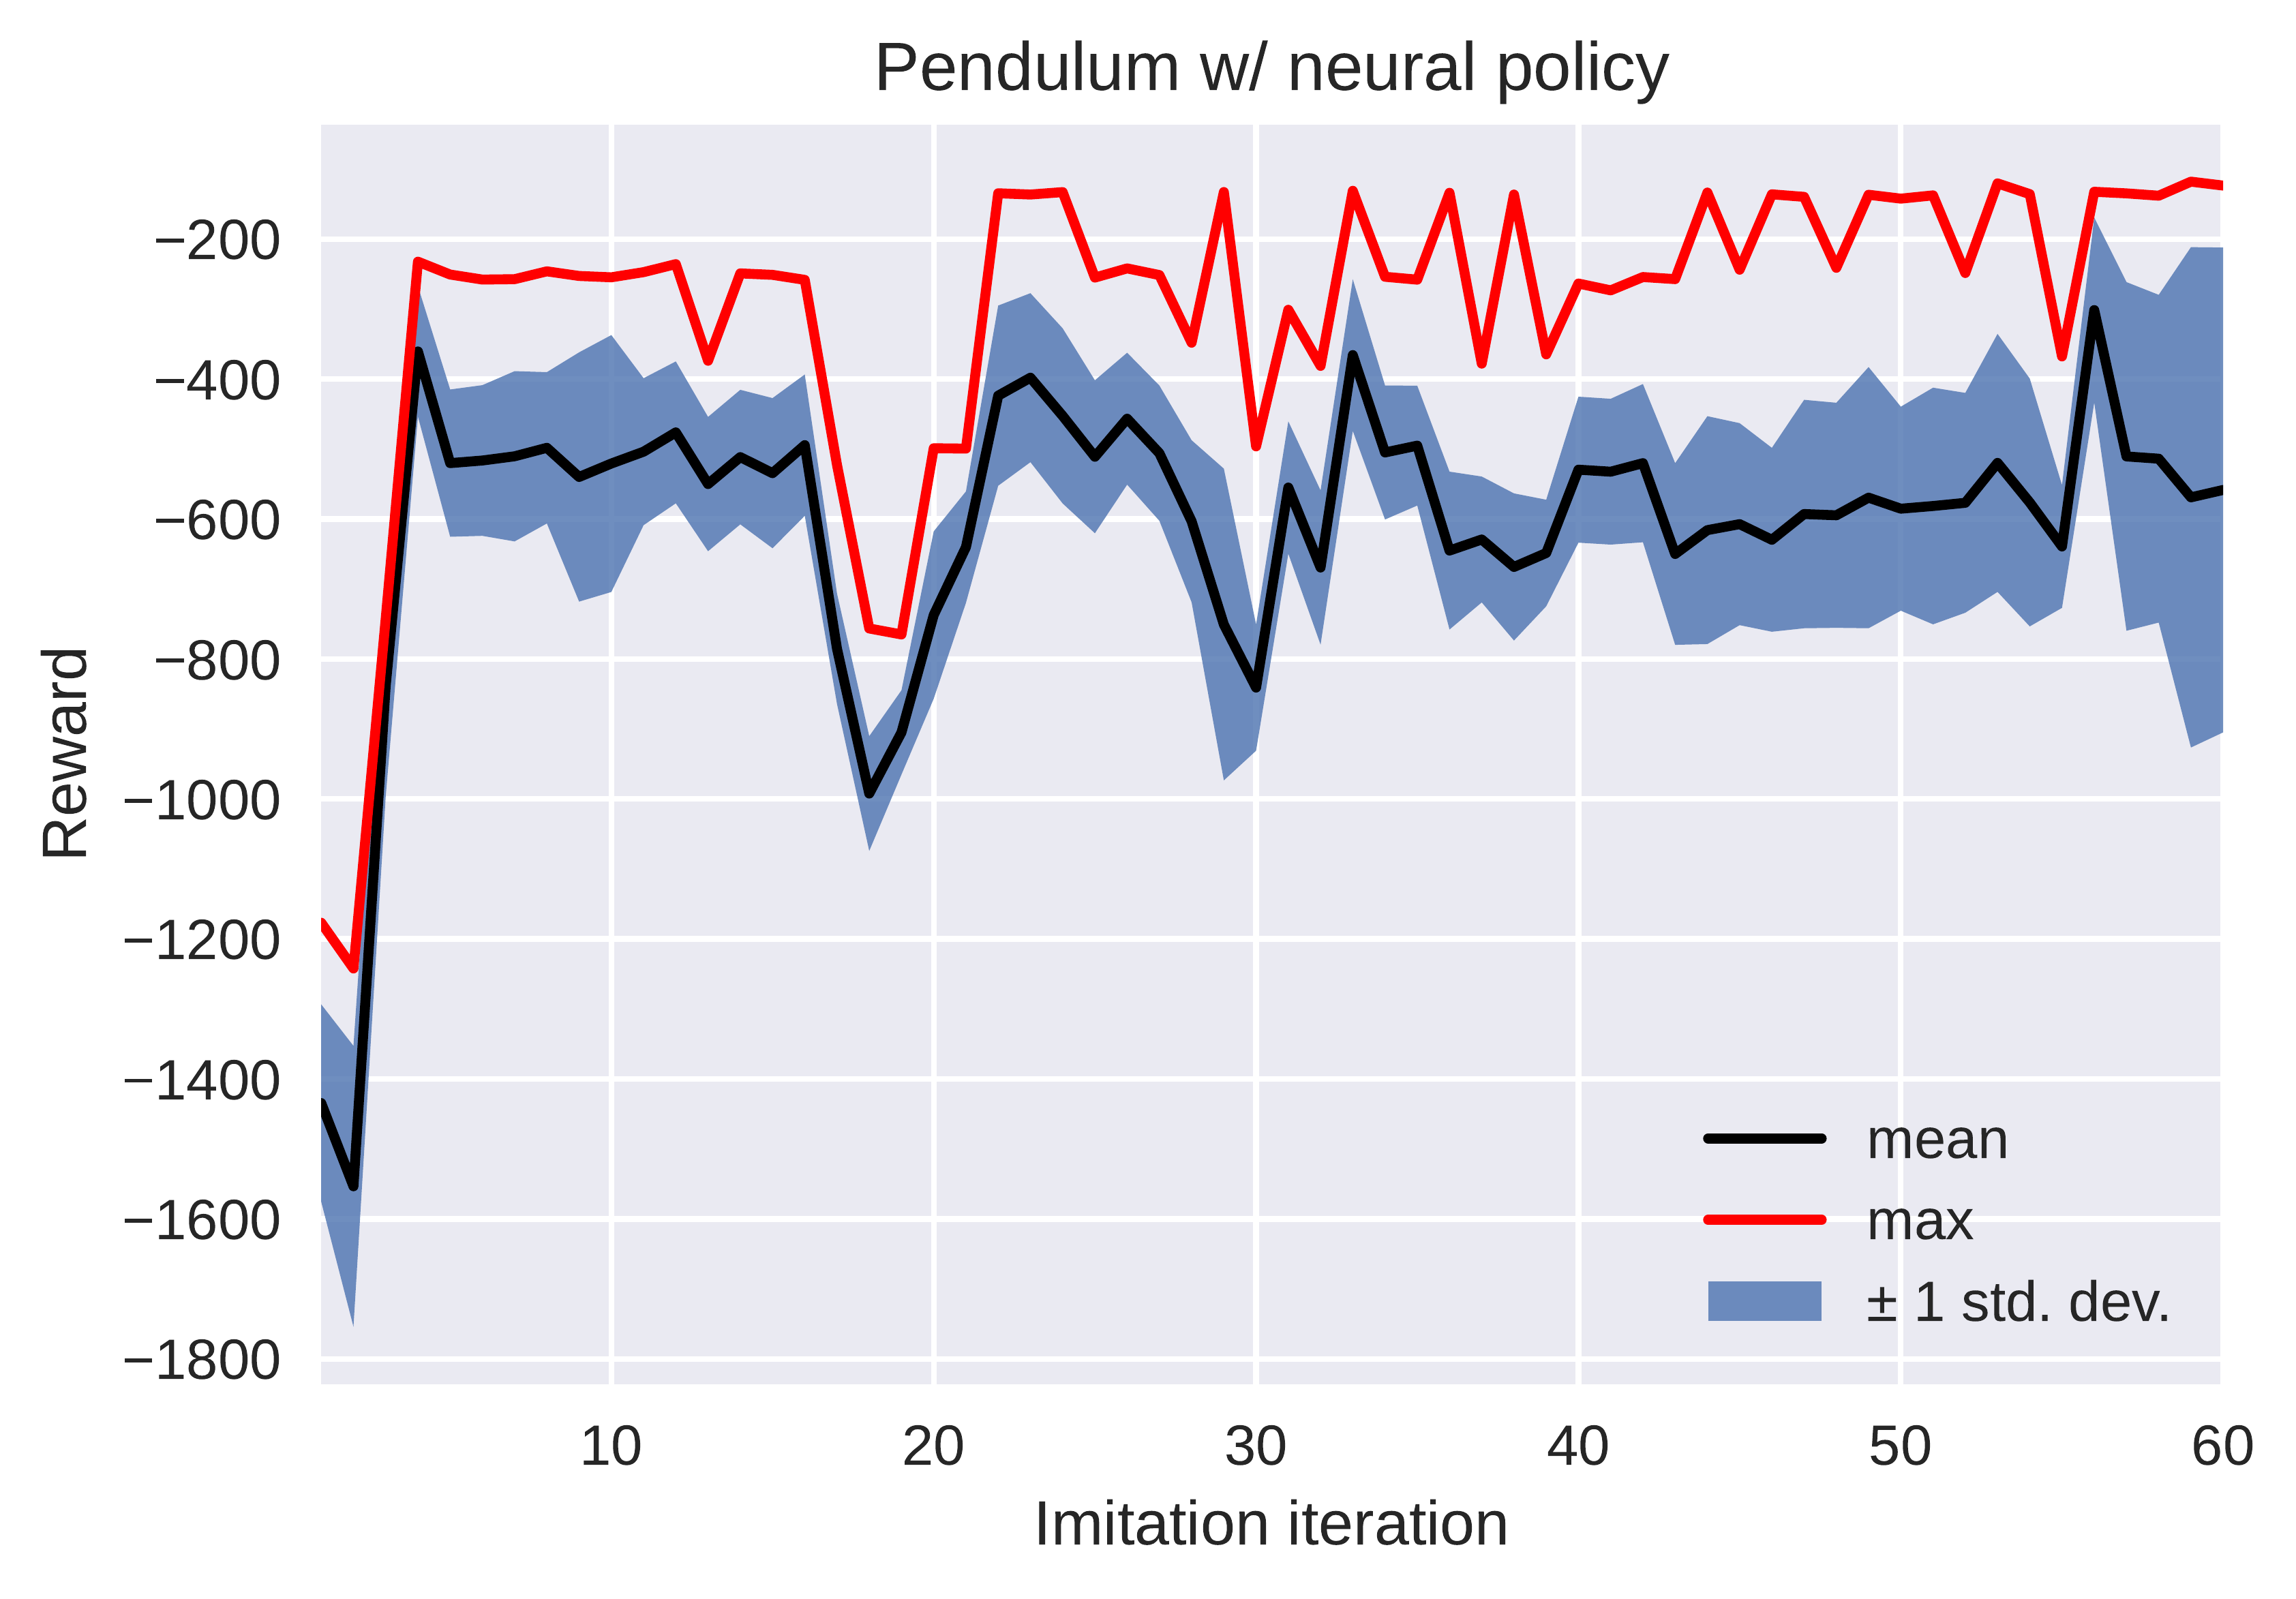
\includegraphics[width=0.37\textwidth]{images/performance.png}
      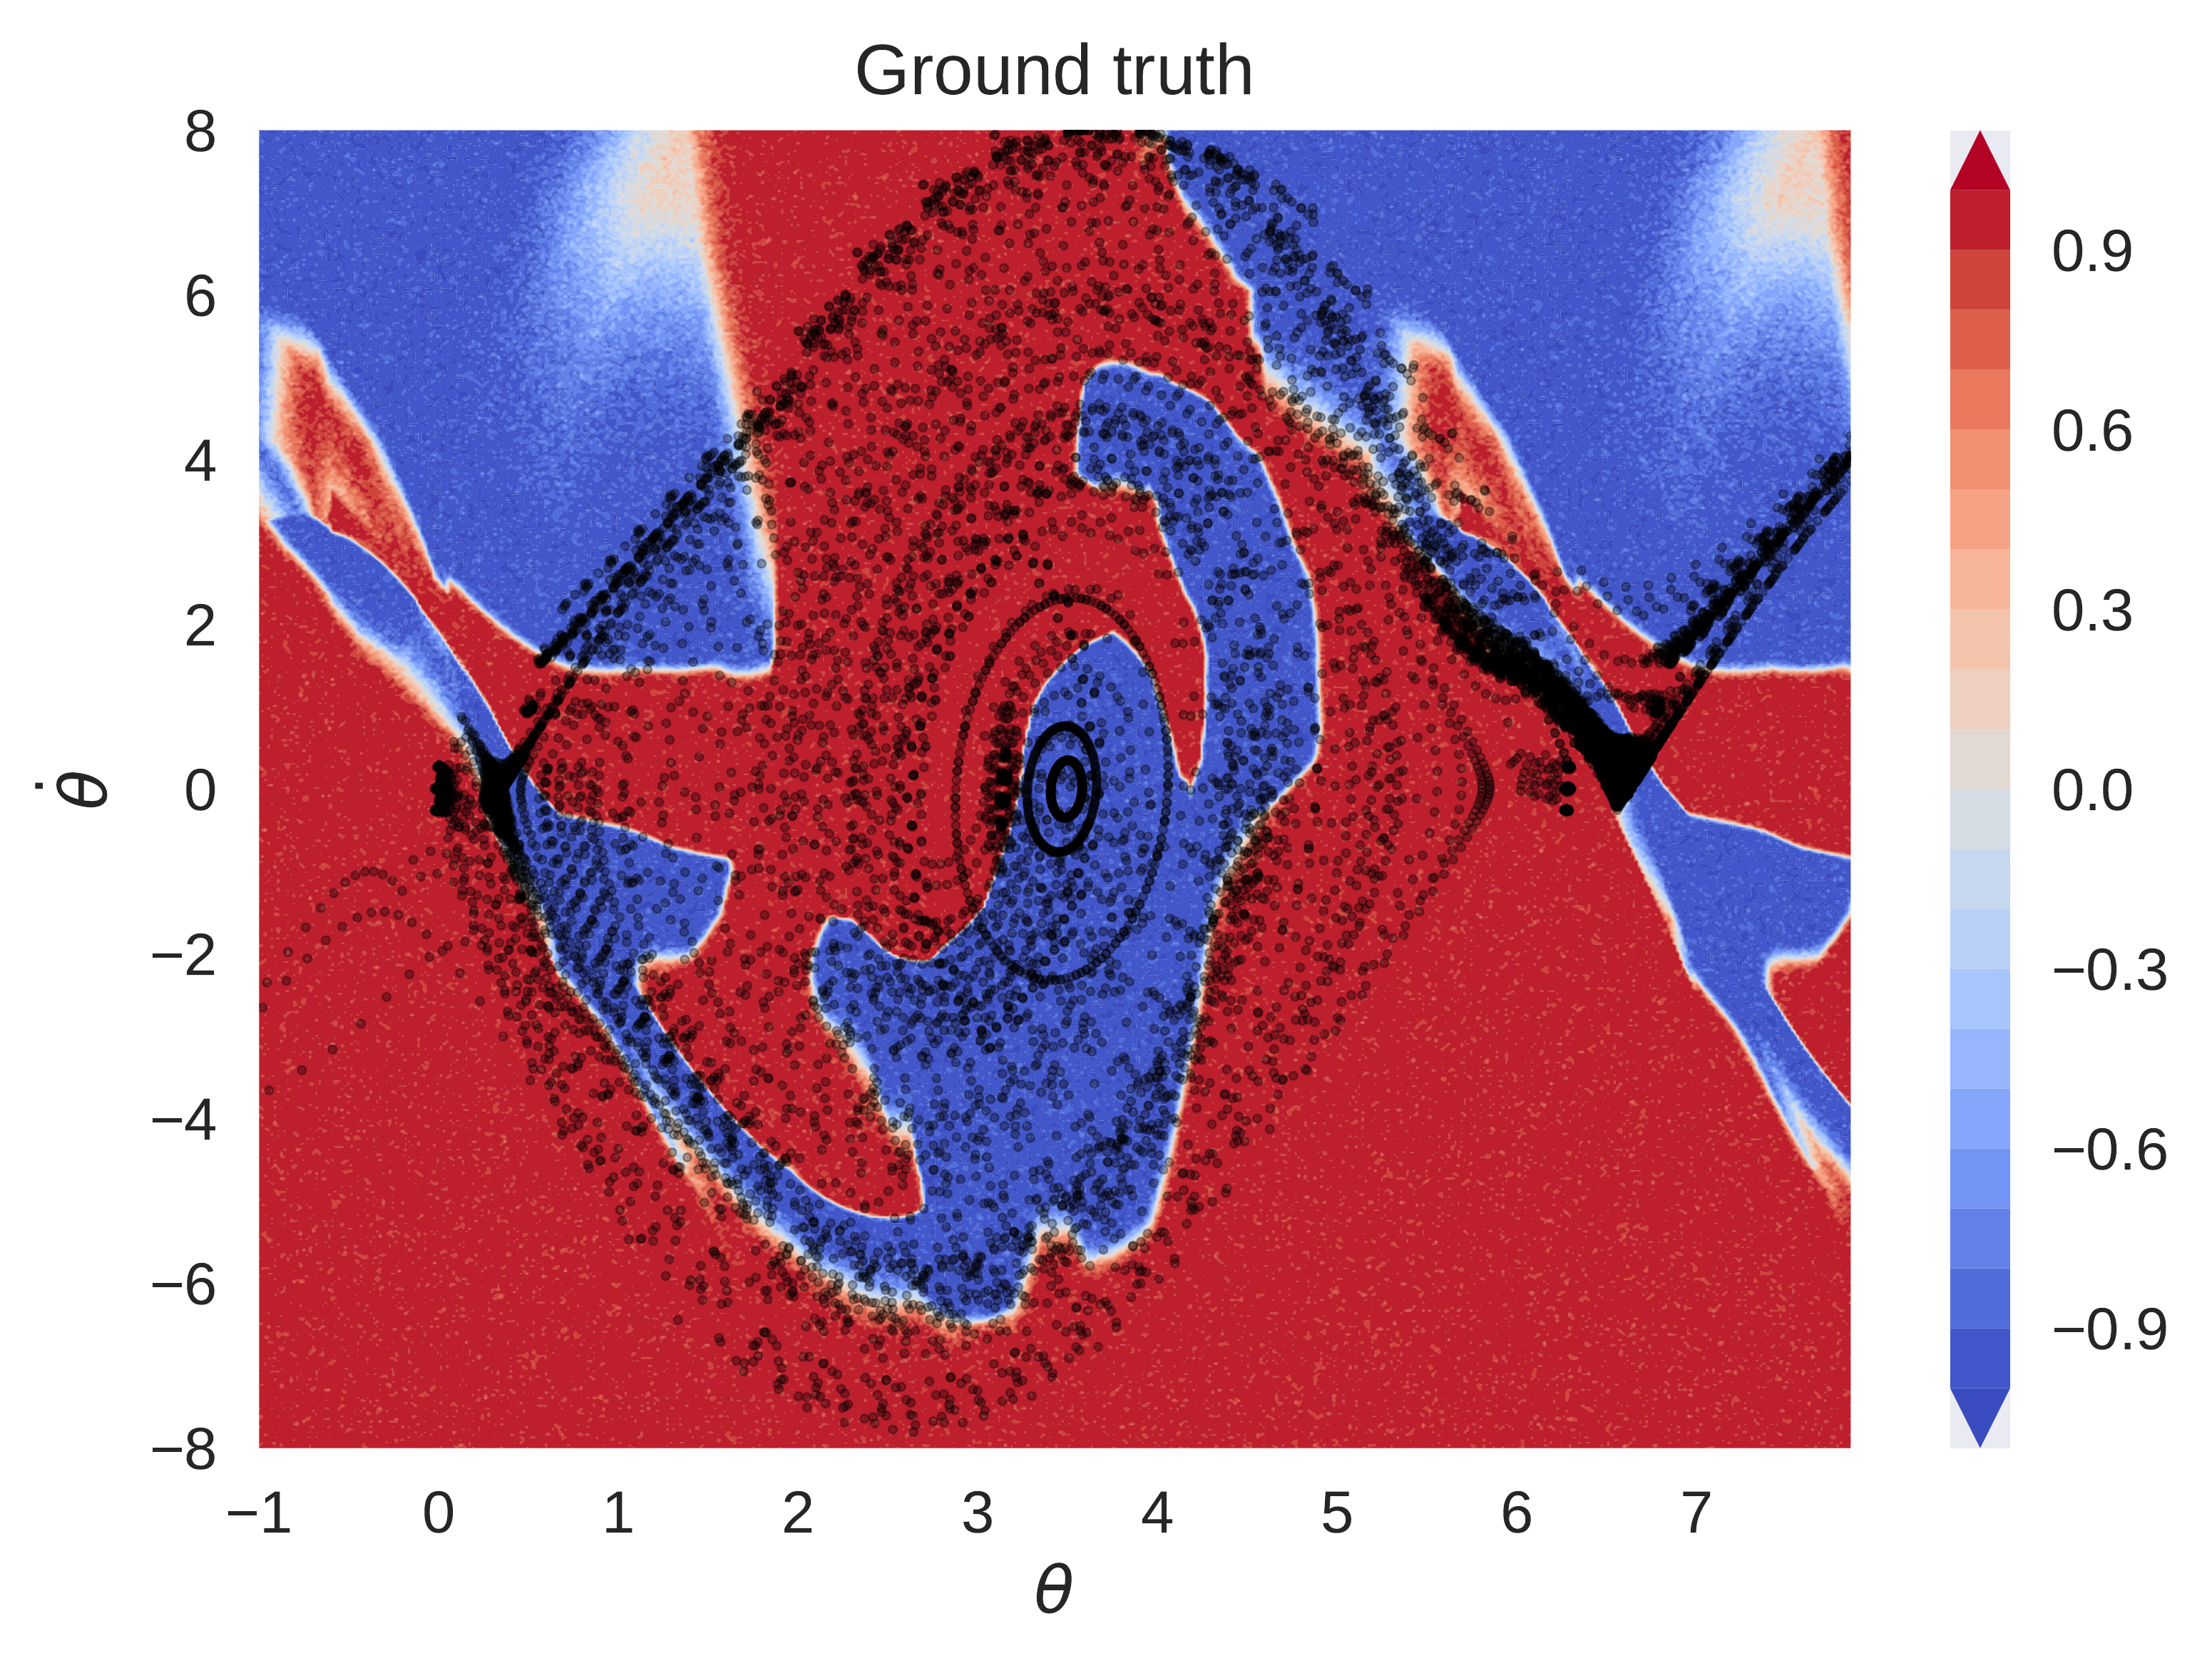
\includegraphics[width=0.37\textwidth]{images/groundtruth.png}
      
      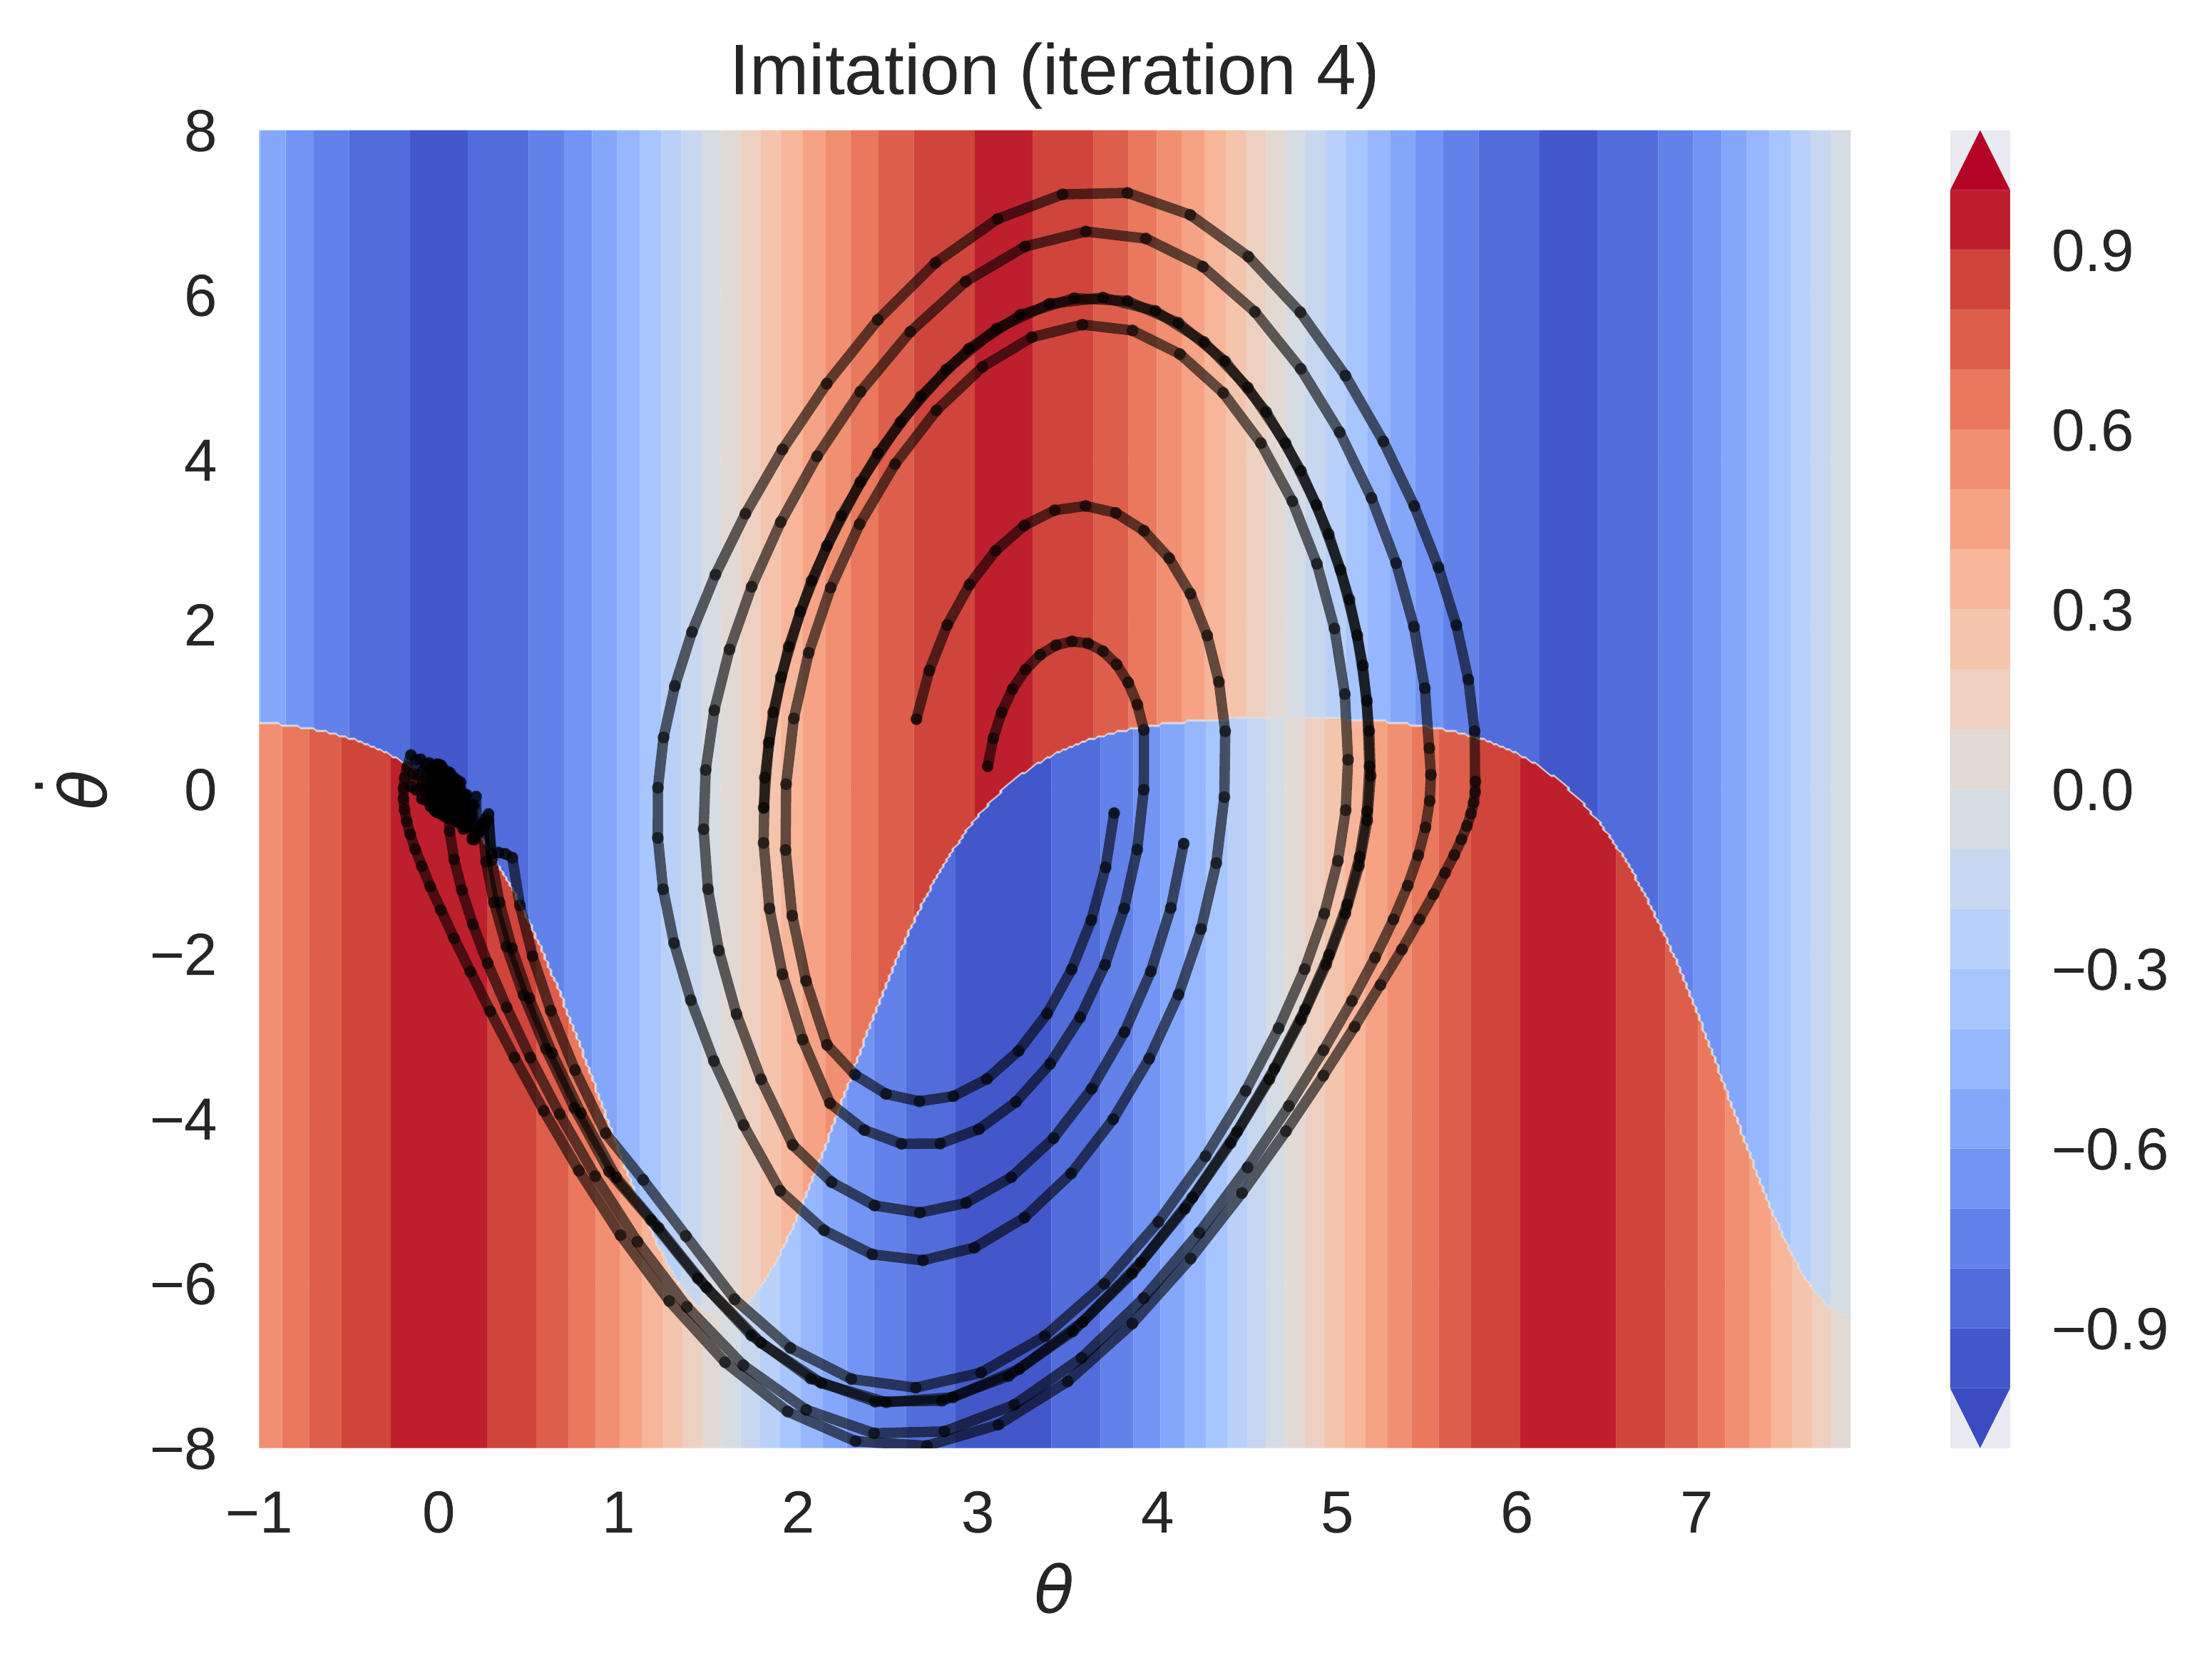
\includegraphics[width=0.37\textwidth]{images/imitation4.png}
      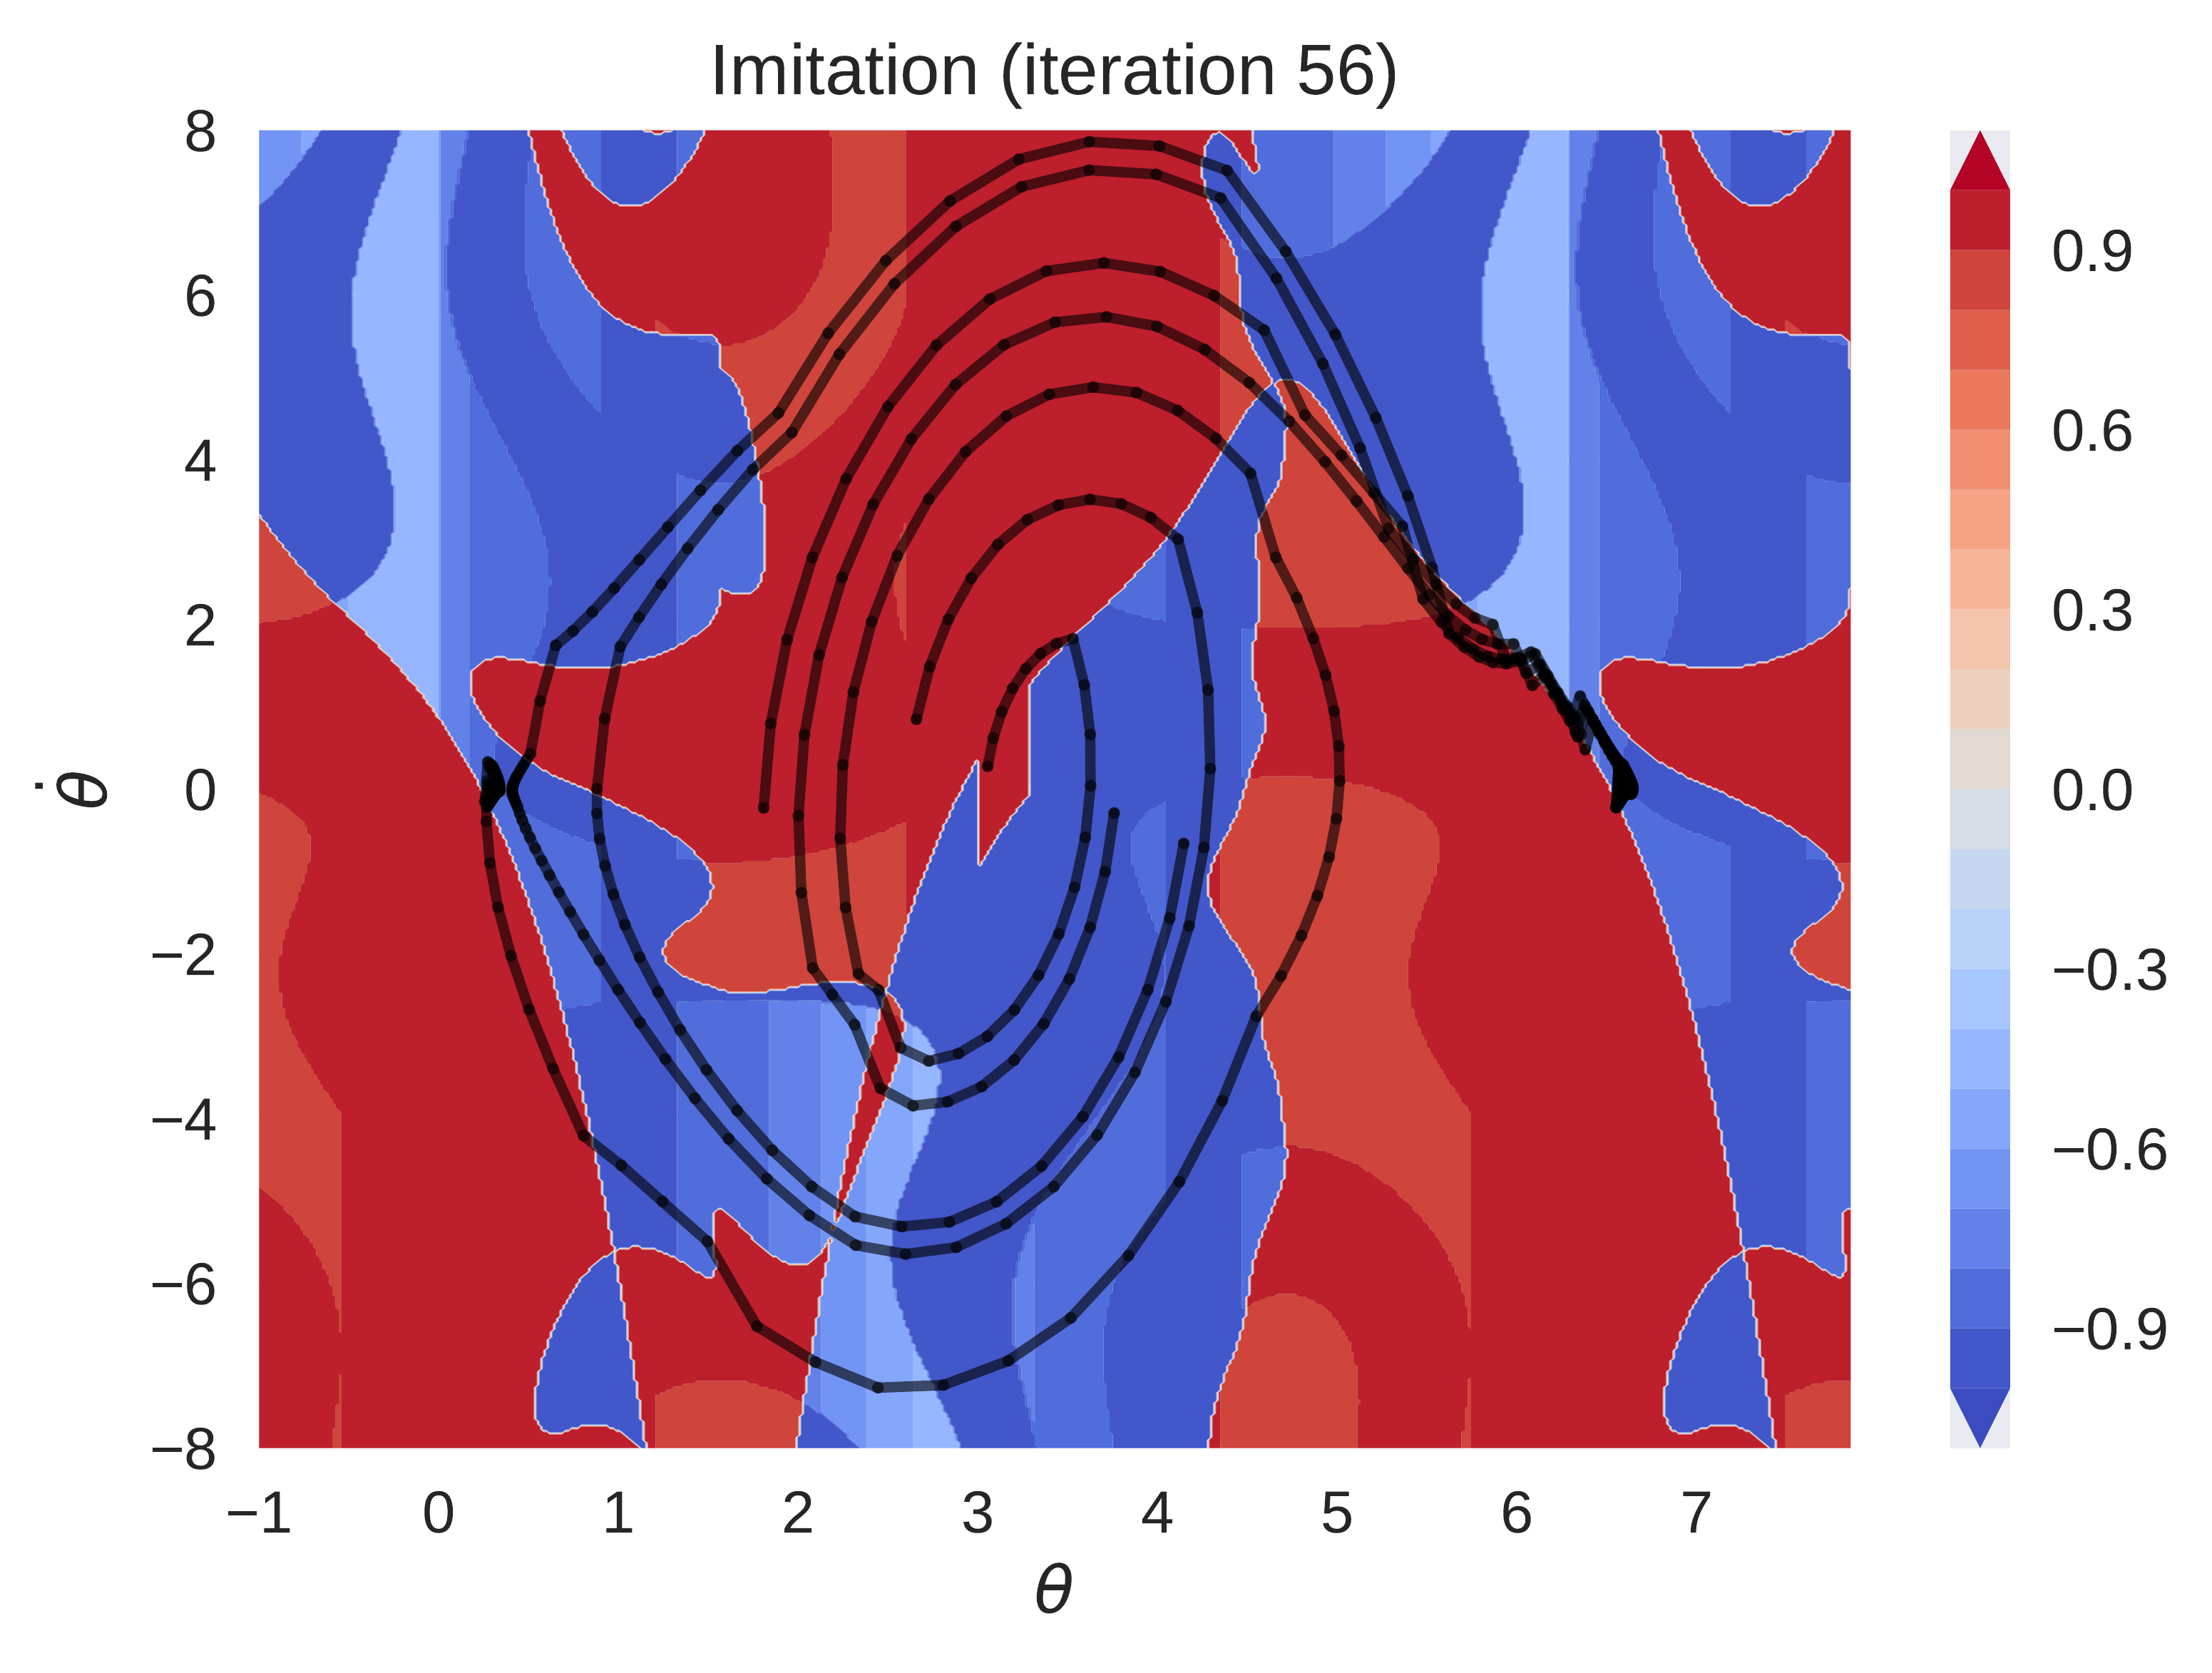
\includegraphics[width=0.37\textwidth]{images/imitation56.png}
    \end{figure}
    
\end{frame}

\begin{frame}{Summary}
    \begin{itemize}
        \item The Imitation-Projected Programmatic Reinforcement Learning framework integrates reinforcement learning with structured policy representations.
        \item We propose an extension to the framework, which we argue is key when scaling to more complicated structured spaces such as DSLs.
        \item Our experiments show that, despite using a simple local search heuristic which generates quite a few semantically identical candidates, interesting and/or complex solutions can be discovered across multiple iterations of interactive search.
    \end{itemize}
\end{frame}

\begin{frame}{Future work}
\begin{itemize}
    \item Improve neighborhood efficiency, e.g. keep track of templates and symmetries.
    \item Integrate synthesis and learning steps, i.e. outer loop.
    \begin{itemize}
        \item How do we take advantage of discovered programs in the following reinforcement learning updates?
    \end{itemize}
    \item Examine policy decompositions and corresponding representations/DSLs.
    \begin{itemize}
        \item High-dimensional input processing.
        \item Decision making.
        \item Low-level control.
        \item Others?
    \end{itemize}
    \item Can certain reinforcement learning algorithms help discover structure better than others?
\end{itemize}
\end{frame}